\section{Longitudinal control}
\label{longitudinal_control}
We have already discussed and the dynamics (lateral and longitudinal) of vehicles and how to develop models to mathematically capture these dynamics. 
In this chapter we would like to go through the concepts of longitudinal vehicle control to regulate the speed of our self-driving car. 
Specifically, we will review some of the essential concepts from classical linear time-invariant control, develop a PID control law for the longitudinal vehicle model and combine feedforward and feedback control to improve desired speed tracking. 

\subsection{LTI control \& a PID controller}
Design of the longitudinal speed control underpins all vehicle performance on the road and is one of the fundamental components needed for autonomous driving. 

In this section, we will briefly review some of the basics of linear time-invariant (LTI) control and the PID controller. 

\begin{framed}
\theoremstyle{remark}
\begin{remark}{\textbf{Prerequisites}}

Note that we will have to assume you're familiar with classical control design including the use of transfer functions and the Laplace domain. 
The Laplace transoformation is discussed in the appendix.
\end{remark}
\end{framed}

In module three of this course, we learned how to develop the dynamic and kinematic models for a vehicle based on the bicycle model. 
These models aim to capture how the dynamic system reacts to input commands from the driver such as steering gas and break and how it reacts to disturbances such as wind, road surface and different vehicle loads. 
The effects of the inputs and disturbances on the states such as velocity and rotation rate of the vehicle 
are defined by the kinematic and dynamic models we developed. 

The role of the controller then is to regulate some of these states of the vehicle by sensing the current state variables and then generating actuator signals to satisfy the commands provided. 

\begin{figure}[!htb]
\begin{center}
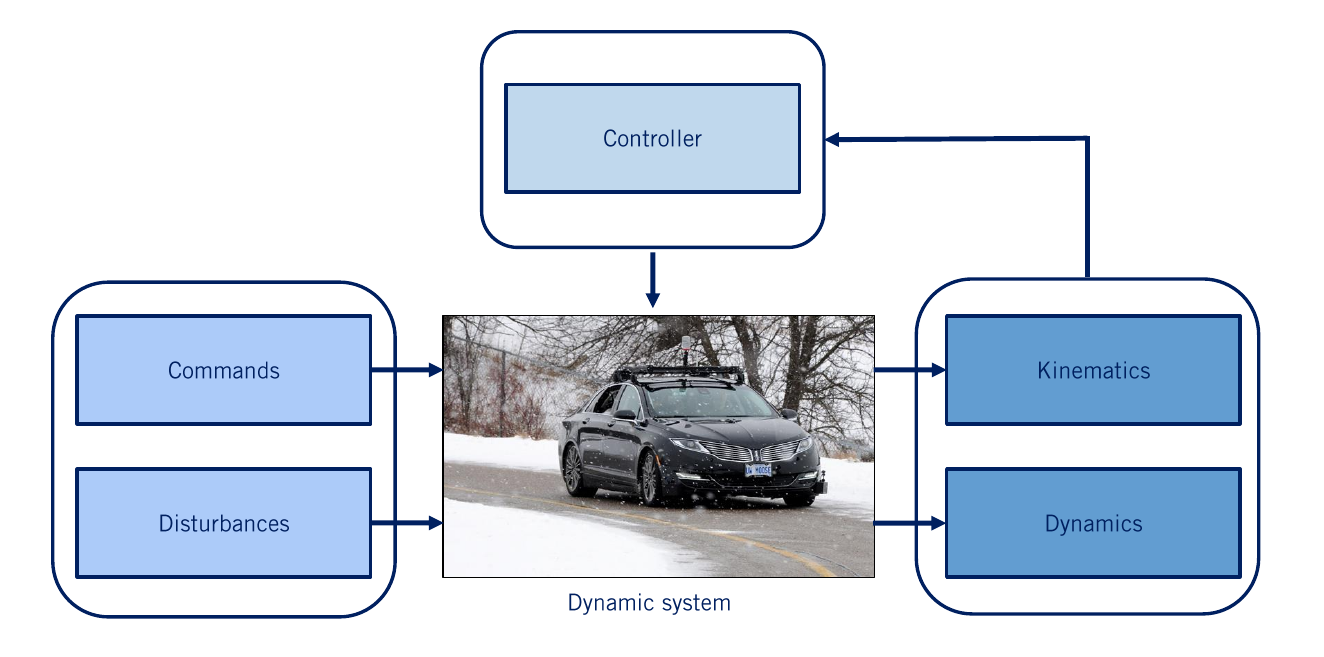
\includegraphics[scale=0.380]{img/longitudinal_control/dynamic_system.jpeg}
\end{center}
\caption{Schematics of Pipe-and-Filter pattern.}
\label{dynamic_system}
\end{figure}

For longitudinal control, the controller sensing the vehicle speed and adjust the throttle and break 
commands to match the desired speed set by the autonomous motion planning system. A typical feedback control loop is shown in figure \ref{feednack_control}. 

\begin{figure}[!htb]
\begin{center}
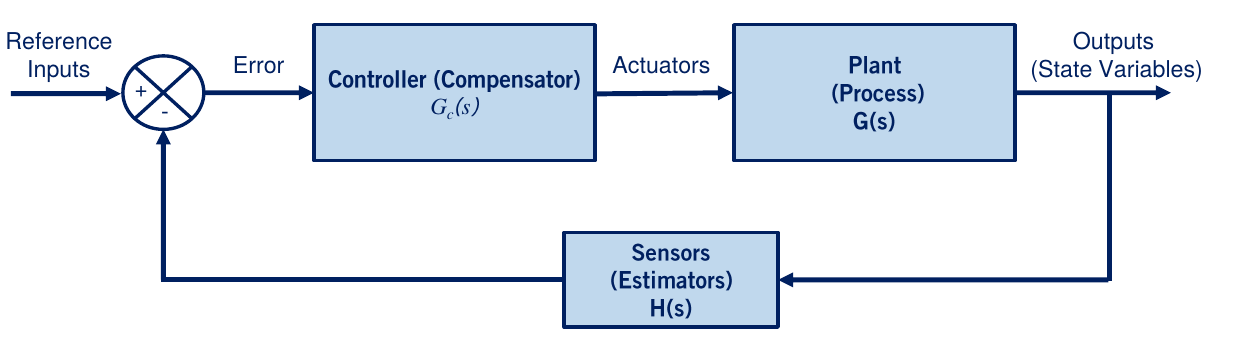
\includegraphics[scale=0.380]{img/longitudinal_control/feednack_control.jpeg}
\end{center}
\caption{Schematic of typical feedback control system.}
\label{feednack_control}
\end{figure}

The plant or process model takes the actuator signals as the input and generates the output or state variables of the system. These outputs are measured by sensors and estimators are used to fuse measurements into accurate output estimates. The output estimates are compared to the desired or reference output variables and the difference 
or error is passed to the controller. 

The controller can be seen as a mathematical algorithm that generates actuator signals so that the error signal is minimized and the plant 
state variables approach the desired state variables. 
The plant model be it linear or nonlinear can be represented in several ways. 
Two of the most common ways are:

\begin{itemize}
\item State-space form which tracks the evolution of an internal state 
to connect the input to the output 
\item Transfer functions which models the input to output relation directly
\end{itemize} 

\begin{framed}
\theoremstyle{remark}
\begin{remark}{}

Note that for transfer functions, the system must be linear and time-invariant.
\end{remark}
\end{framed}

\subsection{Transfer functions}
\label{transfer_functions}

A transfer function $G$ is a relation between inputs $U$ and outputs $Y$ of the system defined in the so called Laplace domain as a function of  the complex variable $s$. 

\begin{equation}
Y(s) = G(s) U(s), ~~ s= \sigma + j \omega
\end{equation}

We use the Laplace transform to go from the time domain to the $S$ domain because it allows for easier analysis of an input-output relation 
and is useful in understanding control performance. 

When working with the transfer functions, the numerator and denominator roots provide powerful insight into the response of a system to input functions. 
The {\textbf{zeros}} of a system are the roots of the numerator and the {\textbf{poles}} of the system are the roots of its denominator. 

Control algorithm design can vary from simple such as constant gain multiplication, lookup tables and linear equations to more detailed methods based on non-linear functions and optimization over finite prediction horizons. Some of the basic and classic controllers include lead-lag controllers and proportional integral and derivative or PID controllers. 


\subsection{PID control}
\label{pid_control} 
We will now go into more detail on the PID control combination as a useful starting point for longitudinal control. More involved control design is also possible and it's particularly useful for non-linear system models, time-varying models, or models with constraints that limit output selection. Nonlinear methods such as feedback linearization, back stepping and sliding mode control  can certainly be applied to self-driving vehicle control problem and will be discussed in another chapter. Optimization-based methods are heavily used in autonomous driving and so we'll look at model predictive control as an example of this group of controllers later on. 

PID control is mathematically formulated by adding three terms dependent on the error function. A proportional term directly proportional to the error E, an integral term proportional to the integral of the error, and a derivative term proportional to the derivative of the error. The constants $K_p$, $K_i$, and $K_d$ are called the proportional integral and derivative gains and govern the response so the PID controller which is denoted by $u(t)$ assuming that the time $t$ it is the input to the plant model. 

\begin{equation}
u(t) = K_P e(t) + K_I \int_{0}^{t}e(t)dt + K_D \dot{e}(t)
\end{equation}

Taking the Laplace transform of the PID control yields the transfer function $Gc(s)$. 
Multiplying by $s$ in the Laplace domain is equivalent to taking a derivative in the time domain and dividing by $s$ is equivalent to taking the integral.By adding these three terms of the PID controller together, we get a single transfer function for PID control. 

\begin{equation}
U(s) = G_c(s)E(s) = ( K_P + \frac{K_I}{s} + K_D s)E(s) = (\frac{K_D s^2 + K_Ps + K_I}{s})E(s)
\end{equation}

Note that not all gains need to be used for all systems. If one or more of the PID gains are set to zero, the controller can be referred to as $P$, $PD$ or $PI$. The PID transfer function contains a single pole at the origin which comes from the integral term. It also contains a second-order numerator with two zeros that can be placed anywhere in the complex plane by selecting appropriate values for the gains. PID control design therefore, boils down to selecting zero locations to achieve the desired output or performance based on the model for the plant. There are also several algorithms to tune PID gains, among them, Ziegler Nichols is one of the most popular. 


Closed loop response denotes the response of a system when the controller decides the inputs to apply to the plant model. For a step input on the reference signal we can define the rise time as the time it takes to reach 90 percent of the reference value. The overshoot as the maximum percentage the output exceeds this reference. The settling time as the time to settle to within five percent of the reference and the steady-state error as the error between the output and the reference at steady-state. The effects of each $P$, $I$ and $D$ action are summarized in the following table. 


\begin{center}
 \begin{tabular}{||c c c c c ||} 
 \hline
 Closed loop response & Rise time & Overshoot &  Settling time & Steady state error  \\ [0.5ex] 
 \hline\hline
 Increase $K_P$ & Decrease & Increase & Small change & Decrease  \\ 
 \hline
 Increase $K_I$  & Decrease & Increase & Increase & Eliminate \\
 \hline
 Increase $K_D$ & Small change & Decrease & Decrease & Small change  \\ [1ex] 
 \hline
\end{tabular}
\end{center}

For instance, an increase in $K_P$ leads to a stronger reaction to errors and therefore a decrease in rise time in response to a step change in the reference signal. Similarly, since $K_D$ reacts to the rate of change of the error an increased $K_D$ leads to a decrease in overshoot or the rate of change of error is high. It may simultaneously lead to a decrease in oscillations about the reference and a decreased settling time as a result. Finally, an increase in $K_I$ can eliminate steady-state errors but may lead to increased oscillation in the response. Ultimately, the $P$, $I$ and $D$ gains must be selected with knowledge of the interaction of their effects to adjust the system response to get the right closed loop performance. 

\subsubsection{Example: Spring-mass-dumper system}
Now, let's take a look at the well-known second-order spring-mass damper model as shown in figure \ref{spring_mass_damper_system}. 

\begin{figure}[!htb]
\begin{center}
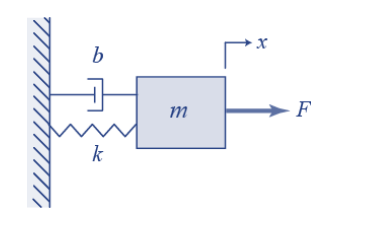
\includegraphics[scale=0.380]{img/longitudinal_control/spring_mass_damper_system.jpeg}
\end{center}
\caption{ system.}
\label{spring_mass_damper_system}
\end{figure}

In this example, we'll first review the transfer function of the proposed dynamic system and then design a PID controller for it. The dynamics of the spring-mass damper system  are modeled by the second order ODE:

\begin{equation}
m\ddot{x} + b\dot{x} + kx = F, ~~ x(0) = 0
\end{equation}

 The system is subjected to the input force $F$ and the output of the model is the displacement of the body $x$. The mass $m$ is connected to a rigid foundation by a spring with spring constant $K$ and a damper with damping coefficient $b$. Now to transform the equation into the $S$ or Laplace domain, we use the Laplace transform and write the second-order equation as follows. 

\begin{equation}
ms^2X(s) + bsX(s) + kX(s) = F(s) 
\end{equation}

This relies on the fact that the derivative in the time domain are multiplications by $s$ in the Laplace domain. Finally, the transfer function is formed which represents the relation between the output $X(s)$ and the input $F(s)$ and is defined as the plant transfer function $G(s)$. 


\begin{equation}
G(s) = \frac{X(s)}{F(s)} = \frac{1}{ms^2 + bs + k} 
\end{equation}

This is a second-order system with two poles defined by the mass spring constant and damping coefficient. To evaluate the system characteristics, we excite the system by using a unit step input. This is normally the first step to evaluate the dynamic characteristics of a plant. For example, the system response $x$ is plotted here for the parameter values given as $m=1$, $b =10$ and $k = 20$. The input is the unit step and $F=1$ and the output is once again $x$. 

The so called open-loop response (since there is no controller applied to the system at this point) of the system
is shown in Figure \ref{open_loop_response_spring_mass_damper}. 

\begin{figure}[!htb]
\begin{center}
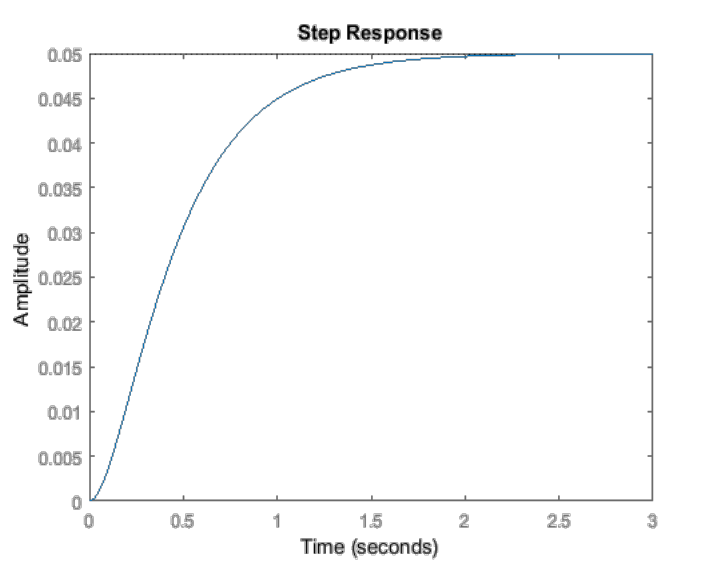
\includegraphics[scale=0.380]{img/longitudinal_control/open_loop_response_spring_mass_damper.jpeg}
\end{center}
\caption{Open loop response for spring-mass-damper system.}
\label{open_loop_response_spring_mass_damper}
\end{figure}

If a controller is added to the plant and the output of the model is measured and compared with the desired output or reference signal, then the response of the system is called the closed loop response. For unity feedback, the sensor transfer function is assumed to be one and in general it could be any transfer function. The closed loop transfer function given here can be performed from the transfer functions of the controller and the plant. For those of you who have studied classical feedback control, you'll know that the poles of the open-loop system define the characteristics of the closed-loop response. You may have also seen root locus Bode and Nyquist design techniques which can be used to select controllers that meet specific output specifications. 

Let's look at the step response for a few different PID controllers. Figure \ref{closed_loop_spring_mass_damper_system}
summarizes some of the options we could use. 

\begin{figure}[!htb]
\begin{center}
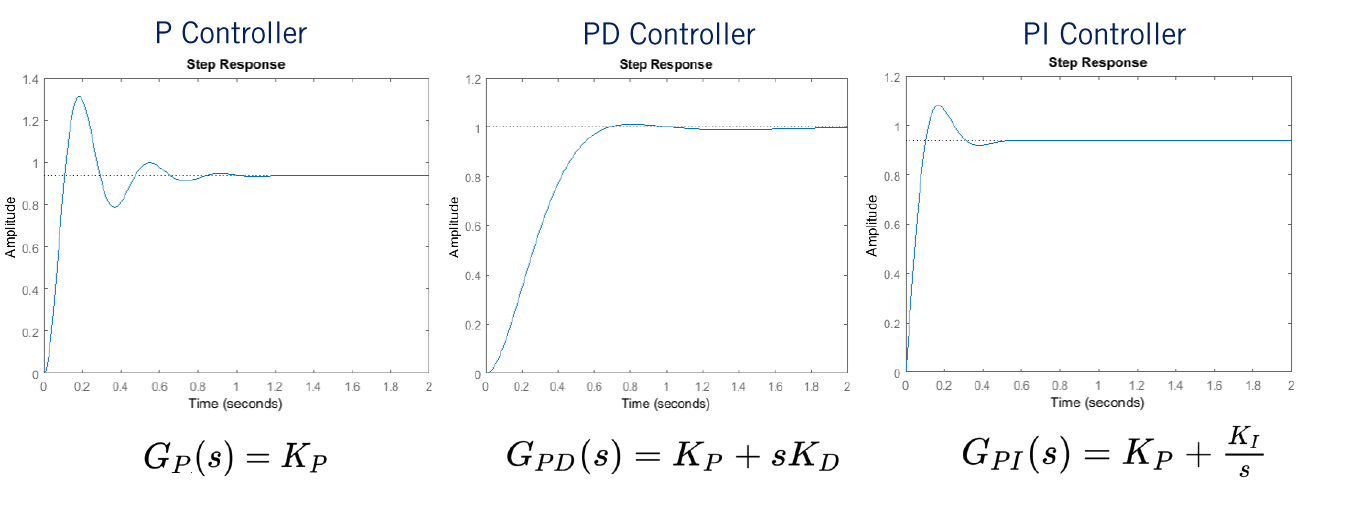
\includegraphics[scale=0.380]{img/longitudinal_control/closed_loop_spring_mass_damper_system.jpeg}
\end{center}
\caption{Closed loop responses for spring-mass-damper system for various PID controllers.}
\label{closed_loop_spring_mass_damper_system}
\end{figure}

The dashed horizontal line represents the reference or desired output and the controllers goal is to keep the actual output close to this reference. In the first example, the step responses for pure proportional control of the spring-mass damper system. In the $P$ controller response, we see a fast rise time, significant overshoot and prolonged oscillation leading to a long settling time. Adding derivative control improves the step response in terms of overshoot and settling time but slows down the rise time. Adding the integral term instead maintains a short rise time and is able to reduce oscillations and overshoot leading to a fast settling time as well. The simple $PI$ control is an excellent design for the spring-mass damper system. 

Including all three PID terms in the controller, leads to even more flexibility in designing the step response. By carefully tuning the controller gains, we can use the benefits of all three to eliminate overshoot and still maintain very short rise and settling times. As can be seen in Figure \ref{full_pid_spring_mass_damper_system}, the system approaches the reference at much more quickly without any overshoot with PID control.  

\begin{figure}[!htb]
\begin{center}
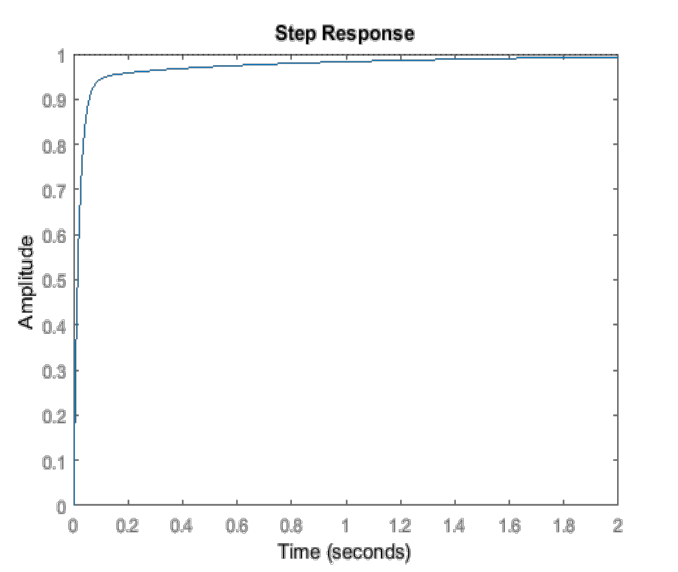
\includegraphics[scale=0.380]{img/longitudinal_control/full_pid_spring_mass_damper_system.jpeg}
\end{center}
\caption{PID control of  spring-mass-damper system with unit step input.}
\label{full_pid_spring_mass_damper_system}
\end{figure}

\subsection{Longitudinal control with PID}
\label{longitudinal_control_pid}

The previous section touched upon the desing of PID controllers and classical control design. In this section, we want to apply PID control to our longitudinal vehicle model. 
Concretely, we will define the full vehicle planning and control architecture and design a PID-based controller for regulating to a set reference speed as in cruise control. 

Let's take a closer look at the vehicle control architecture and how it fits into the overall autonomy software stack. 
We can divide the structure into four sections as seen in Figure \ref{architecture_vehicel_control_strategy}. 

\begin{figure}[!htb]
\begin{center}
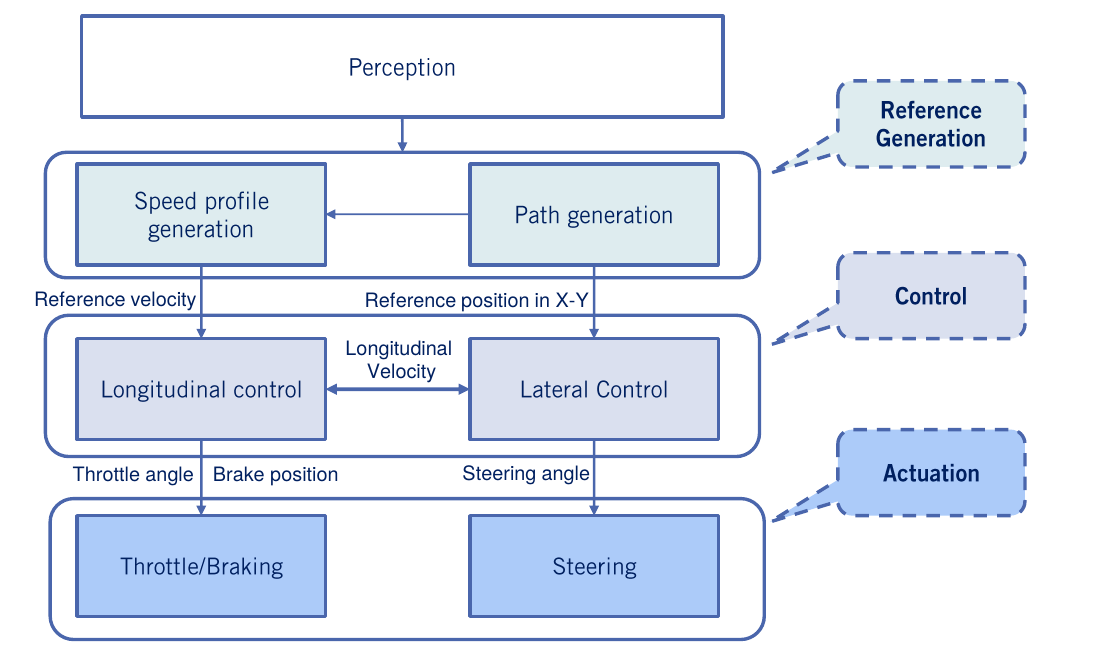
\includegraphics[scale=0.380]{img/longitudinal_control/architecture_vehicel_control_strategy.jpeg}
\end{center}
\caption{Architecture for vehicle control strategy.}
\label{architecture_vehicel_control_strategy}
\end{figure}

These sections are connected to each other. The first section is the perception of the road and the environment. 
This perception is captured by sensors and generates the input references for our system. 
In the second layer, we have both path generation and speed profile generation, which in automotive circles is referred to as the drive cycle. 
These profiles are generated through the motion planning process. 
The path and the speed profiles are the reference inputs needed by our controllers. For longitudinal control, define the set point's, acceleration and deceleration that we'd like to be able to track precisely. For both the lateral and longitudinal control of an autonomous vehicle, the only task that needs to be performed is to follow the plan as precisely as possible, and thereby minimize the error between the actual and reference path and speed. All other tasks required for autonomous driving or done by other parts of the system. 
Finally, the controllers generate the input commands or actuator signals for the vehicle. 

As we've seen in the previous module, these include the steering for the lateral control and the throttle and break commands for longitudinal control. 
Let's look at an example of longitudinal vehicle control. 
One of the most well-known and commonly available control applications in automotive control is cruise control operating at highway speeds. 
A cruise control system performs the function of maintaining a fixed reference speed using throttle commands, and accelerating or decelerating to a new reference speed as requested by the driver. 
When the vehicle is subjected to different loads and resistances, the throttle angle will be changed by the cruise controller accordingly. 
Many systems now exist with expanded capabilities such as the adaptive cruise control, which can vary the reference point based on measurements of a 
lead vehicle and semi autonomous systems, like traffic jam assist, which can operate throughout the vehicle 
speed range and create spacing gaps for merging vehicles. 
These extended examples require additional controller designed to handle the wider range of operating points. 
Figure \ref{cruise_control}, shows the block diagram of the cruise controller and plant vehicle model as a closed loop system 
designed to keep the vehicle velocity close to the reference velocity. 


\begin{figure}[!htb]
\begin{center}
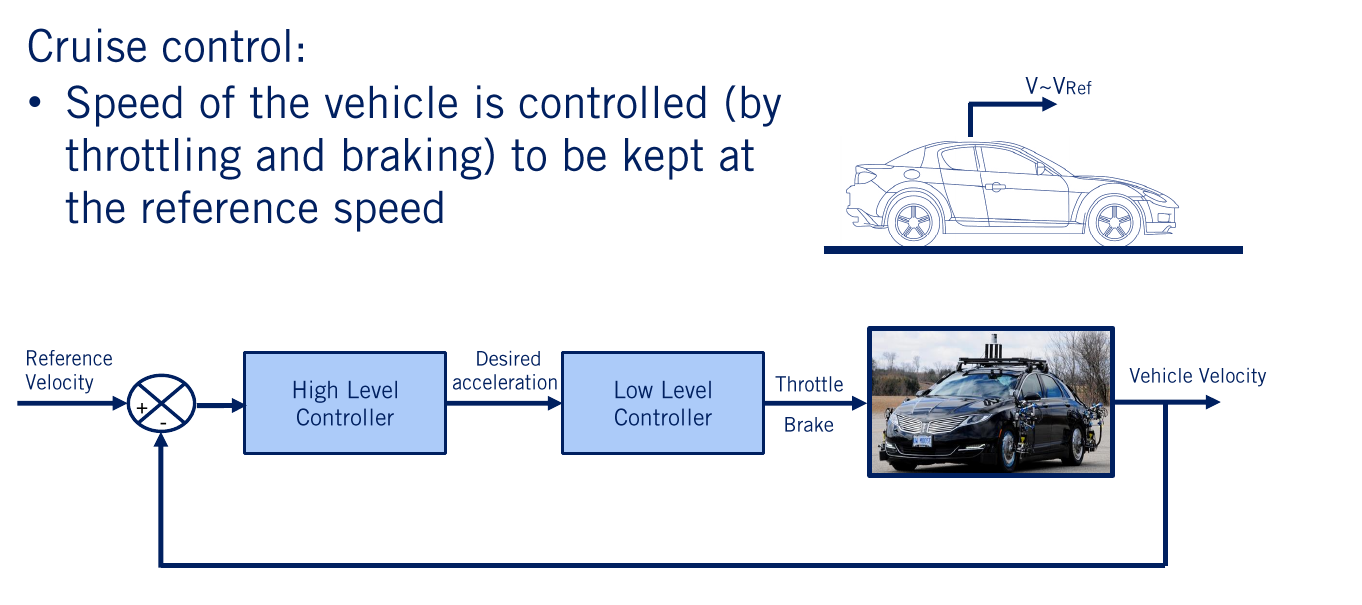
\includegraphics[scale=0.380]{img/longitudinal_control/cruise_control.jpeg}
\end{center}
\caption{Block diagram for cruise control.}
\label{cruise_control}
\end{figure}

The controller can be split into two levels; a high level and a low level controller. 
Although the low level controller is not essential to the control task. 
The high level controller takes the difference between the set point velocity and the vehicle actual velocity, 
and generates the desired vehicle acceleration to close the gap. 
The low-level controller gets the vehicle acceleration and generates a throttle or breaking actuation to track the reference acceleration. 
In practice, this two-stage approach allows us to go beyond just PID control and impose limits or profiles directly on the accelerations that are requested of the vehicle in order to maintain speed. 
It also allows us to separate the use of engine maps we studied in the previous module for generating a desired torque given the engine state from the cruise control input response. 

\subsubsection{High level controller}
\label{high_level_controller}

Let's take a closer look at the high level controller. The upper level or high level controller determines how much acceleration is needed at each time step based on the velocity error. Let's apply a PID controller here, which is expressed in the continuous time domain. 

\begin{equation}
\ddot{x}_{des} = K_P(\dot{x}_{ref}-\dot{x}) + K_I\int_{0}^{t}(\dot{x}_{ref}-\dot{x})dt + K_D\frac{d(\dot{x}_{ref}-\dot{x})}{dt}
\end{equation}
where $K_P, K_I$ and $K_I$ are the control gains.

The input to the high level controller is the velocity error,$\dot{x}_{ref}-\dot{x}$ , and the output is the vehicle's desired acceleration $\ddot{x}_{des}$. In the previous section, we learned how to design a PID controller and studied how the different gains affect performance of the controller. 

To implement such a controller in software, we discretize the controller, changing the integral to a summation over a fixed length time steps. The derivative term can be approximated with the finite difference over a fixed time step if either the reference acceleration or the estimated vehicle acceleration is not available. 

\subsubsection{Low level controller}

The low-level controller generates the throttle and breaking signals to follow the desired acceleration calculated by the high-level controller. In designing a low-level controller, we make some assumptions to simplify our problem. We assume that only throttle is needed to manage the speed of the vehicle during cruise control, and that the driver will take over if breaking is required to avoid an incident. We assume that we are operating in gear three or higher such that the torque converter is locked, meaning that torque from the engine passes directly through the transmission without loss, and we assume that the tire slip angle and ratio are negligible as cruise control motions are typically gentle. The low-level controllers seeks to generate the desired acceleration from the high level controller by increasing or decreasing the torque produced by the engine. This is controlled by the throttle angle, but is governed by the power train dynamics and the engine map, making it a nonlinear problem that can be a challenge for classic control methods. 

Instead, the desired acceleration is translated to a torque demand, and the torque demand is then converted to a throttle angle command. Recall from the previous module that we developed a second-order ordinary differential equation to describe the acceleration of the vehicle in terms of the difference between the engine torque and the load torque. 
We can rearrange this equation to solve for the desired engine torque, given known load torques and the desired acceleration of the vehicle. Then, the steady-state engine map, which is generated in testing the engine at different operating points can be used to determine the throttle angle needed to produce the amount of torque demand required, see Figure \ref{engine_torque_to_throttle_angle}. 


\begin{figure}[!htb]
\begin{center}
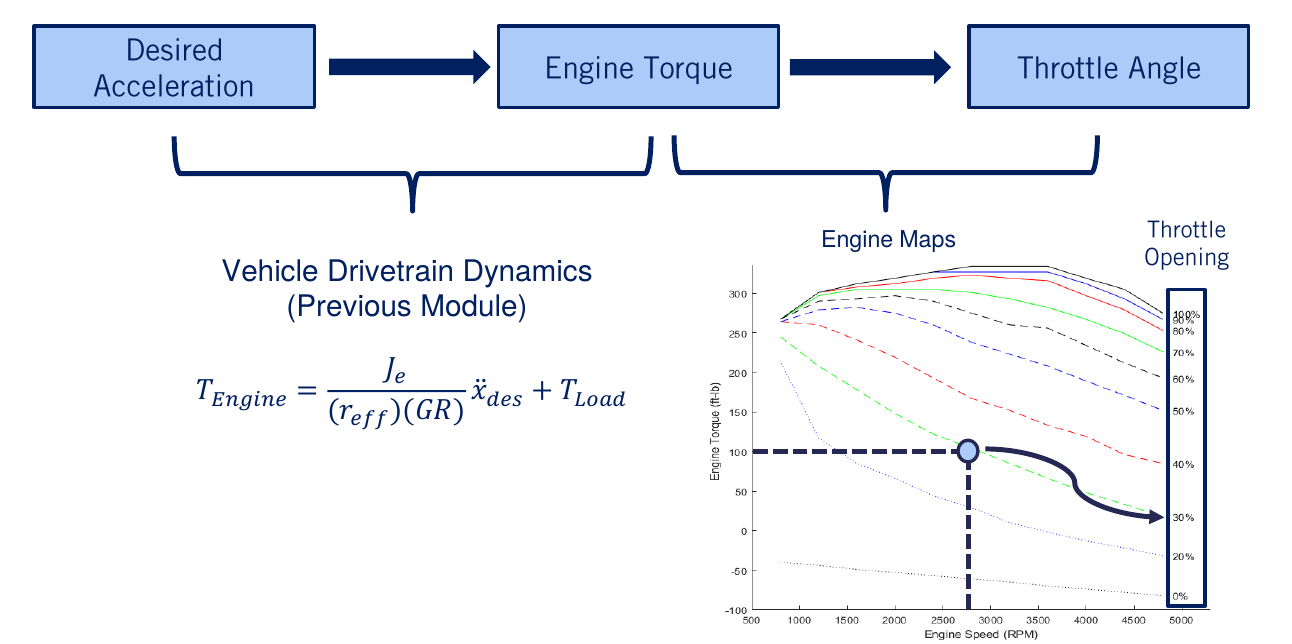
\includegraphics[scale=0.380]{img/longitudinal_control/engine_torque_to_throttle_angle.jpeg}
\end{center}
\caption{Engine torque to throttle angle.}
\label{engine_torque_to_throttle_angle}
\end{figure}

In these standard maps, the desired engine torque and the current engine RPM define the required throttle position, and can be interpolated if needed. 

This approach is a data-driven approximation, but it works quite well in practice. The approximation comes from the fact that the data points in the map are steady-state points while the power train is continuously changing its operating point to meet the current driving conditions. Finally, we can put the pieces of our vehicle controller together and simulate the control response to a step change in desired speed of our dynamic vehicle models with PID controllers. 

The PID gains are tuned by trial and error so that the vehicle speeds follow the reference velocity of 30 meters per second or a 108 kilometers per hour. In the results plot, on the left, we see the throttle opening as a percentage, which is the commanded throttle for the vehicle. On the right, we see how the actual velocity evolves over time, and reaches the reference velocity after a settling time. Because of the engine map non-linearity, we see some interesting artifacts in the vehicle response as it closes in on the reference speed. 

\begin{figure}[!htb]
\begin{center}
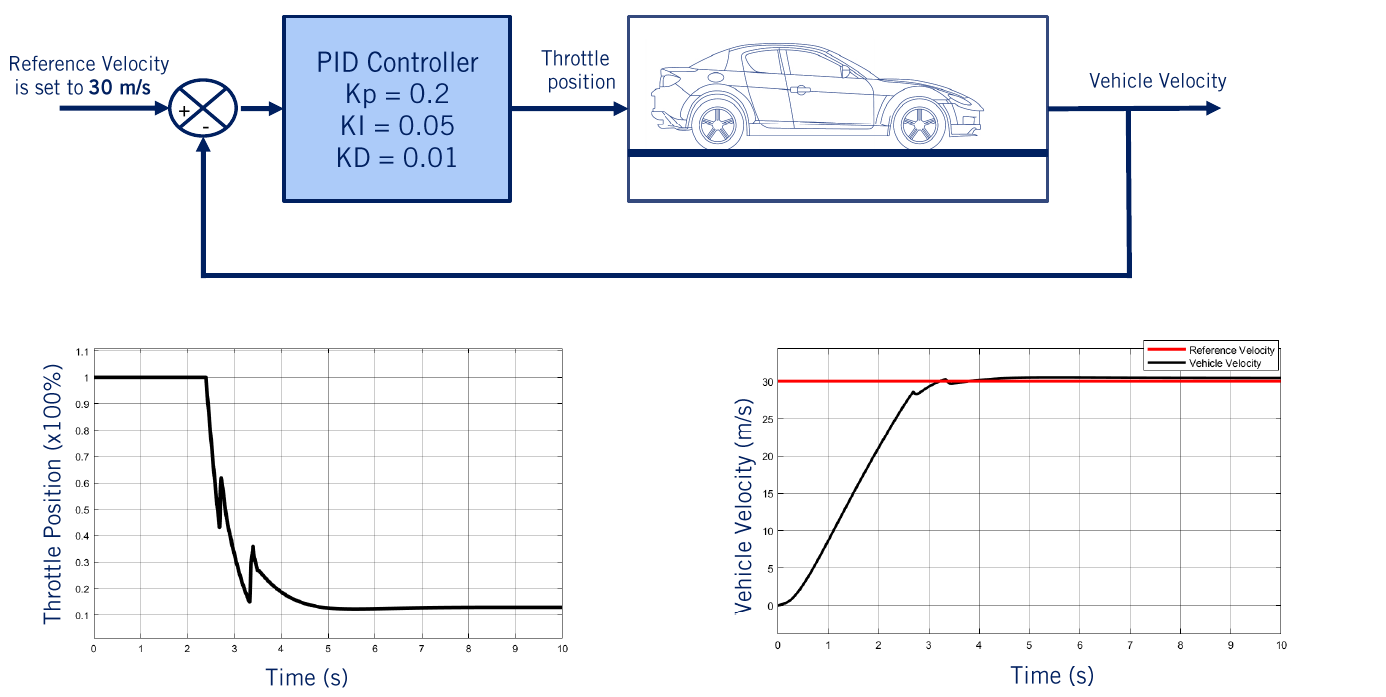
\includegraphics[scale=0.380]{img/longitudinal_control/simulation_example.jpeg}
\end{center}
\caption{Simulation example.}
\label{simulation_example}
\end{figure}


\subsection{Feedforward control design}

In the last section, we saw how to build
a feedback controller for the longitudinal speed tracking problem that used PID
control to generate acceleration commands together, with a low level controller
to define throttle and brake inputs. In this section, we will modify our control architecture
to incorporate feedforward commands, which will improve tracking performance,
particularly in dynamic maneuvers. Specifically, we will see how to
integrate both feedforward and feedback control into a combined
control architecture. We will then apply this architecture
to longitudinal vehicle control. 

\subsubsection{Feedback vs feedforward}

Let's first  compare the feedback
versus feedforward block diagrams. These are shown in Figure \ref{feedback_vs_feedforward_control}. 
\begin{figure}[!htb]
\begin{center}
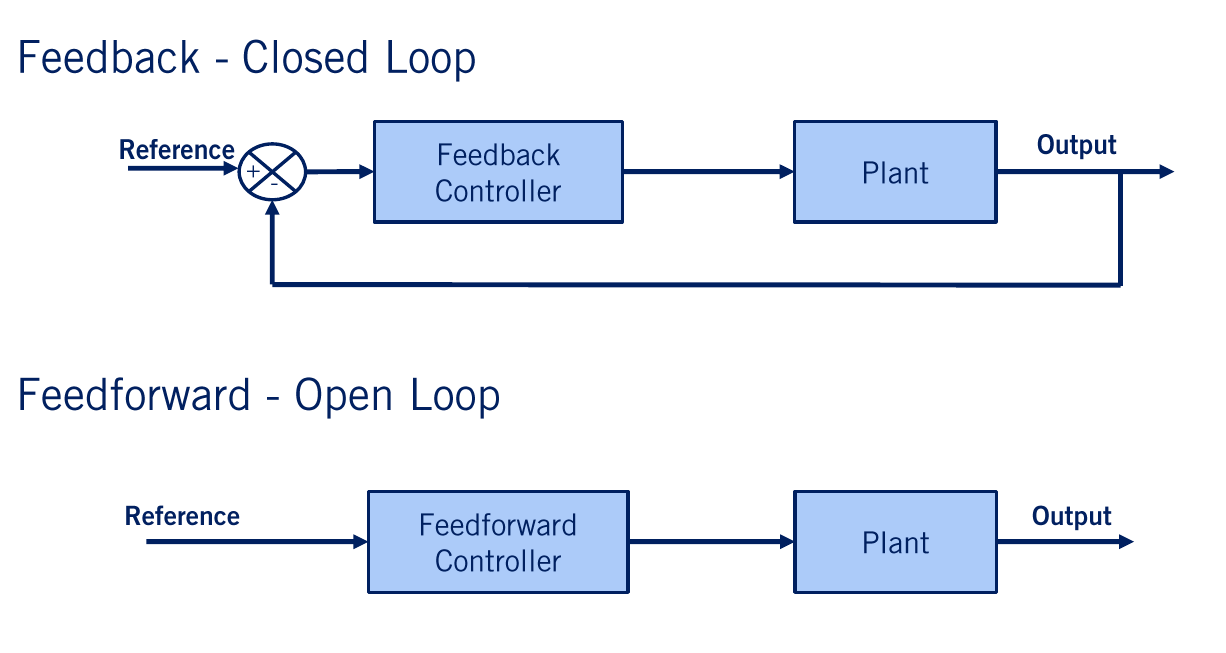
\includegraphics[scale=0.380]{img/longitudinal_control/feedback_vs_feedforward_control.jpeg}
\end{center}
\caption{Feedforward vs feedback block diagrams.}
\label{feedback_vs_feedforward_control}
\end{figure}
The feedback block diagram shows the typical closed loop structure, where the current output is
compared to a reference signal. The error between the two is fed into the feedback controller, which generates the input to the plants. The feedforward block diagram shows an open loop structure, where the reference signal is directly
fed into the feedforward controller, which again, generates the inputs to the plant. Feedforward controllers create their plant inputs by modeling the plant process, as we did in chapter \ref{vehicle_kinematics_and_dynamics}, and applying the appropriate inputs directly. 


In many applications, both feedforward and feedback controllers are combined in order to improve the system performance. 
Figure \ref{feedback_and_feedforward_control_architecture} shows the block diagram of a typical feedback, feedforward control structure. 
\begin{figure}[!htb]
\begin{center}
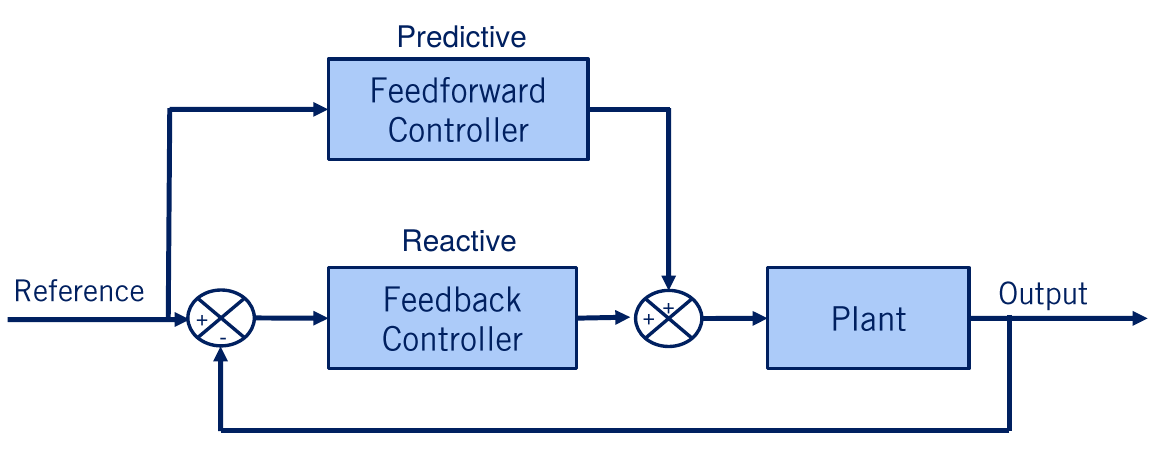
\includegraphics[scale=0.380]{img/longitudinal_control/feedback_and_feedforward_control_architecture.jpeg}
\end{center}
\caption{Combination of feedforward and feedback controllers.}
\label{feedback_and_feedforward_control_architecture}
\end{figure}

You can think of feedforward control as
providing the necessary inputs expected to keep the plant tracking its reference
signal, and the feedback controller correcting for errors that result
from either disturbances or inaccuracies in the plant model
used by the feedforward controller. The input to the plant is simply
the addition of the feedforward and the feedback inputs. 

In summary, the main
reason that both feedback and feedforward controllers are used to control a system
is that on the one hand  feedforward controllers provide a predictive response as they produce
a reference output to achieve a particular tracking response, particularly when
the required inputs are non-zero. On the other hand, feedback controllers provide
a reactive response, which eliminates control errors due
to the disturbances as they occur. The combination of feedback and feedforward control is widely used because
of this complementary relationship. Since autonomous vehicles require
non-zero steering commands to maintain a constant radius turn and a constant
throttle or brake command to maintain constant speed or deceleration rates,
feedforward commands are extremely beneficial in improving
tracking performance in automated driving. 

\subsubsection{Vehicle speed control}

Now let's take a look at the combined
feedback and feedforward controllers to generate vehicle actuation for
longitudinal speed control. The reference speed or drive cycle is
defined by a higher level planner. It is desirable that the vehicle
follows the reference velocity precisely. The reference velocity is the input
to the feedforward block, and the velocity error is the input to
the feedback or PID control block. Both controllers produce two vehicle
actuation signals, the throttle and the brake commands, see Figure \ref{speed_control}. 

\begin{figure}[!htb]
\begin{center}
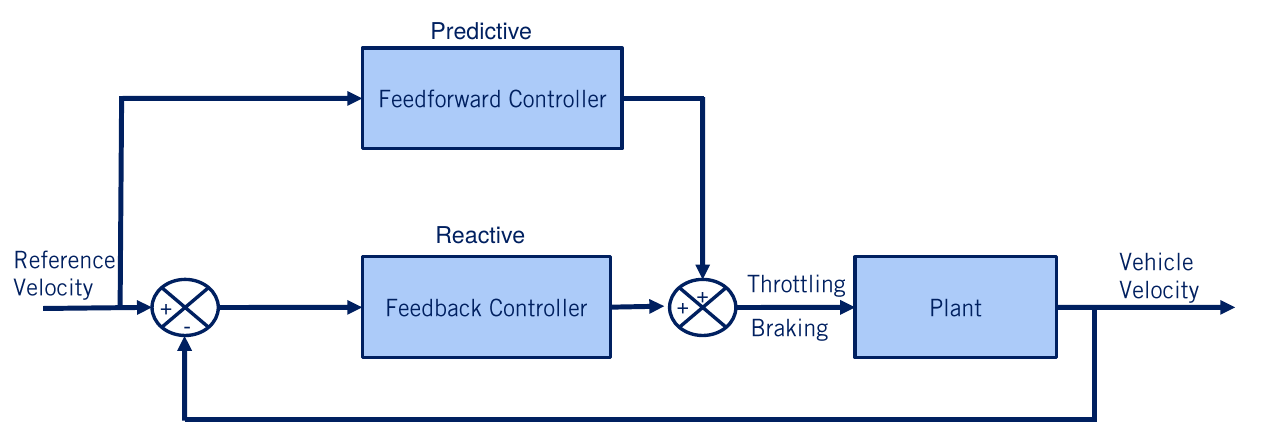
\includegraphics[scale=0.380]{img/longitudinal_control/speed_control.jpeg}
\end{center}
\caption{Controller architecture for speed control.}
\label{speed_control}
\end{figure}

Note that there is no low-level controller
included in the block diagram in Figure \ref{speed_control}, as we had in the pure PID feedback
control. The role of the low-level controller
achieving the desired acceleration through the use of a mapping from
accelerations to engine commands is now going to be handled
by the feedforward block. The feedforward block gets only
the reference signal as input, and its primary objective is to accurately
set the inputs of the plant. 

In order to  do this, we can convert the entire
longitudinal dynamics model into a fixed lookup table or reference
map, that maps the reference velocity to the corresponding actuators signals
assuming the vehicle is at steady state. This feedforward approach works
well at steady state, but ignores the internal dynamics
of the vehicle powertrain. We must also rely on the current
vehicle state estimate to resolve some of the forces and
dynamic models used. Let's look at the steps needed
to develop the actuator commands from a feedforward lookup table. 


\begin{figure}[!htb]
\begin{center}
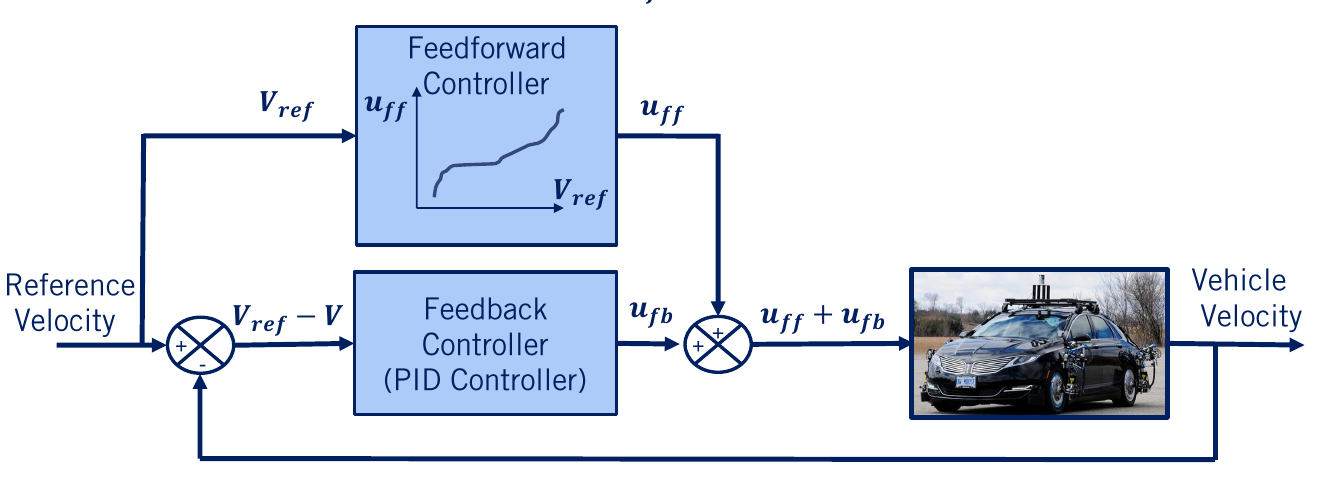
\includegraphics[scale=0.380]{img/longitudinal_control/controlled_actuators.jpeg}
\end{center}
\caption{Controlled actuators.}
\label{controlled_actuators}
\end{figure}

In our example, we are interested in following
the reference velocity at each time step. Based on the kinematic relationship
between the vehicle's speed and the wheel angular speed, we can calculate
the wheel angular speed needed. The wheel angular speed is related
to the engine angular speed, or engine RPM, through the gear
ratios from the transmission, differential and final drive. So we can now compute the engine RPM corresponding to the required wheel angular speed all through the kinematic relationships
defined in the modeling module. Assuming steady state operation,
the dynamics of the powertrain says that the engine torque must be equal to the
total load torque acting on the vehicle. The source of the load torque
is aerodynamic resistance, rolling resistance and
vehicle gravitational resistance. We can compute the combined load torque
using the current state of the vehicle, including its current speed,
and the road slope. We now have a required engine torque and can combine that with the current
engine operating speed in RPM to define the throttle position needed
to generate the required torque. Once again, the engine map is defined for discrete steady state values
of engine torque and RPM and is interpolated as needed, based
on the current vehicle operating point. The above are summarized in Figure \ref{feedforward_table}.


\begin{figure}[!htb]
\begin{center}
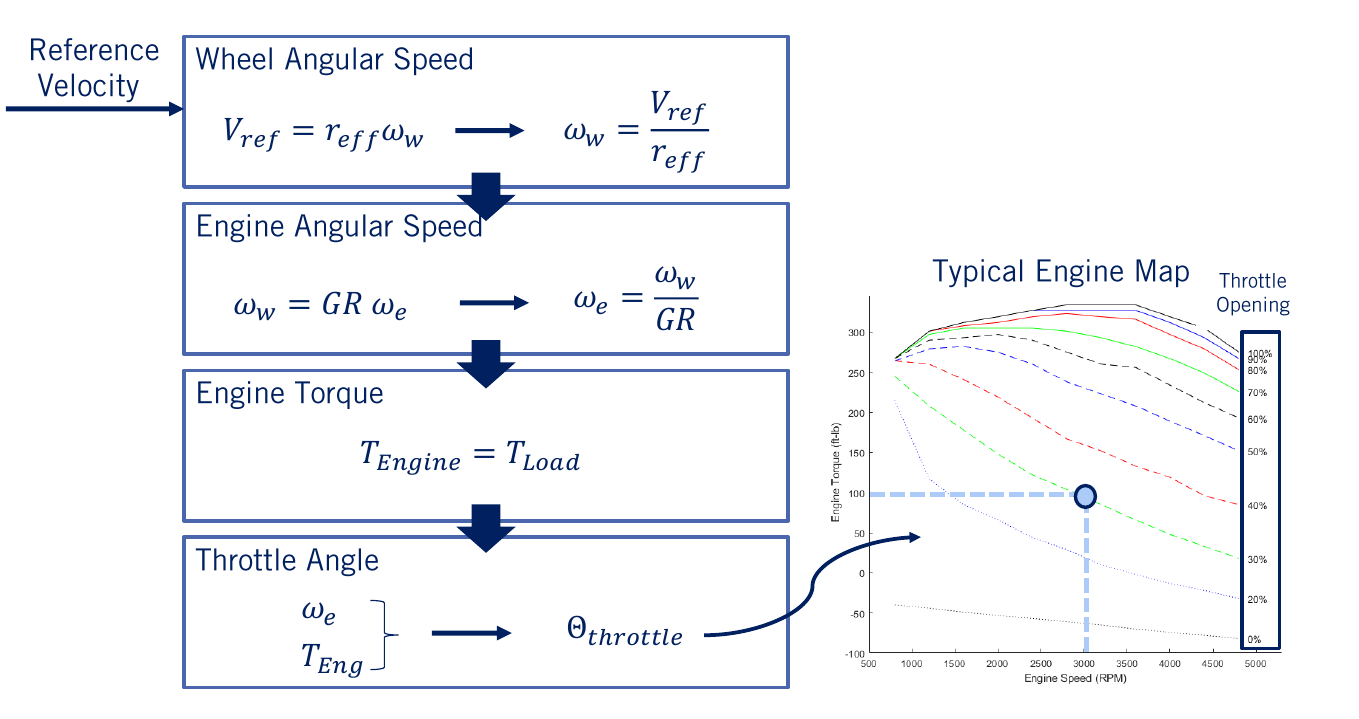
\includegraphics[scale=0.380]{img/longitudinal_control/feedforward_table.jpeg}
\end{center}
\caption{Feedforward table.}
\label{feedforward_table}
\end{figure}

Let's have a look at
the comparison between PID control method described
in the previous section and the combined feedforward, feedback
method we've discussed in this one. We've used the same simulation
parameters as in the previous section, including the engine map and
dynamic model elements. The key difference between
the two responses is visible as the reference speed changes. Because the PID controller needs errors
to exist before it can correct them, its response lags
the feedforward approach, which immediately applies
the relevant input reference values. The feedforward tracking is still not
perfect, however, as the vehicle response is ultimately governed by its inertia, and
the feedforward approach we've presented relies on steady state
modeling of the car. As the feedforward model
becomes more precise, the feedback components can focus
purely on disturbance rejection, and speed profile tracking can be
done with consistent precision. 


\subsection{Questions}
\label{questions_longitudinal_control}

\begin{enumerate}
\item What is the order of the following transfer function?

\begin{equation}
G(s) = \frac{s-10}{s^2 + 2s +1}
\end{equation}
	\begin{enumerate}
		\item  This is the first order transfer function
		\item This is the second order transfer function
		\item This is the third order transfer function
		\item This is the fifth order transfer function
		\item None of the above
	\end{enumerate}
	
\item What are the poles and zeros of the following transfer function?
\begin{equation}
G(s) = \frac{s^2 +3s-10}{s^2 - 2s -12}
\end{equation}
	\begin{enumerate}
		\item  The poles are -3 and 4; the zeros are 2 and -5
		\item The poles are -4 and 3; the zeros are 5 and -2
		\item The poles are 2 and -5; the zeros are -3 and 4
		\item The poles are 5 and -2; the zeros are -4 and 3
		\item None of the above
	\end{enumerate}
\item What might be your action as a system control engineer if you need to increase the overshoot of a control loop system? (Select all that apply)
	\begin{enumerate}
		\item Increase $K_I$
		\item Decrease $K_I$​
		\item Decrease $K_P$ ​
		\item Increase $K_D$ 
		\item Increase $K_P$​
		\item Decrease $K_D$​
	\end{enumerate}
\item Consider the Mass-Spring-Damper System shown in the figure below.

\begin{figure}[!htb]
\begin{center}
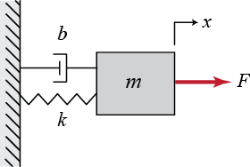
\includegraphics[scale=0.280]{img/longitudinal_control/image_q5_1.png}
\end{center}
\label{image_q5_1}
\end{figure}

As a system control engineer, you constructed the following closed loop transfer function to represent the Mass-Spring-Damper System. 
What is the correct transfer function for this closed loop? 

\begin{figure}[!htb]
\begin{center}
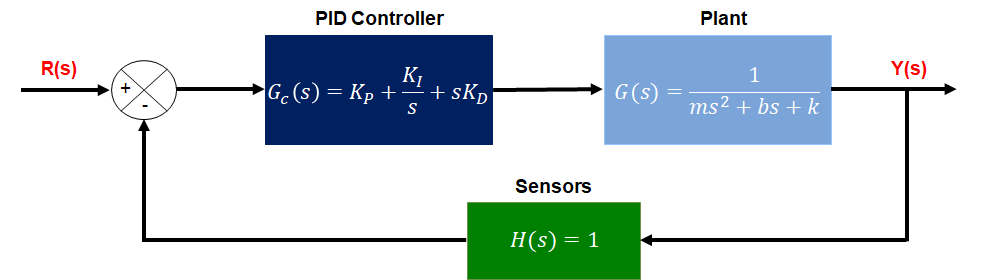
\includegraphics[scale=0.280]{img/longitudinal_control/image_q5_2.png}
\end{center}
\label{image_q5_2}
\end{figure}

\begin{enumerate}
		\item Transformation function 1
		\begin{equation}
			G(s) = \frac{K_Ds^2 + sK_P + K_I}{K_P + \frac{K_I}{s} + K_Ds} 
		\end{equation}
		\item Transformation function 2
		\begin{equation}
			G(s) = \frac{K_P + \frac{K_I}{s} + K_Ds}{K_Ds^2 + sK_P + K_I} 
		\end{equation}
		\item Transformation function 3
		​\begin{equation}
			G(s) = \frac{ms^2 + bs + k + K_P\frac{K_I}{s} + K_Ds}{K_P + \frac{K_I}{s} +K_Ds} 
		\end{equation}
		\item Transformation function 4
		​\begin{equation}
			G(s) = \frac{K_Ds^2 + sK_P + K_I}{ms^3 + (b + K_D)s^2 + (k + K_P)s + K_I} 
		\end{equation}
		\item None of the above
	\end{enumerate}
		
\item You are given the step response of a few different PID controllers using the same gains for the same first order transfer function. 
Determine a possible set of controllers that generated these step responses:

\begin{figure}[!htb]
\begin{center}
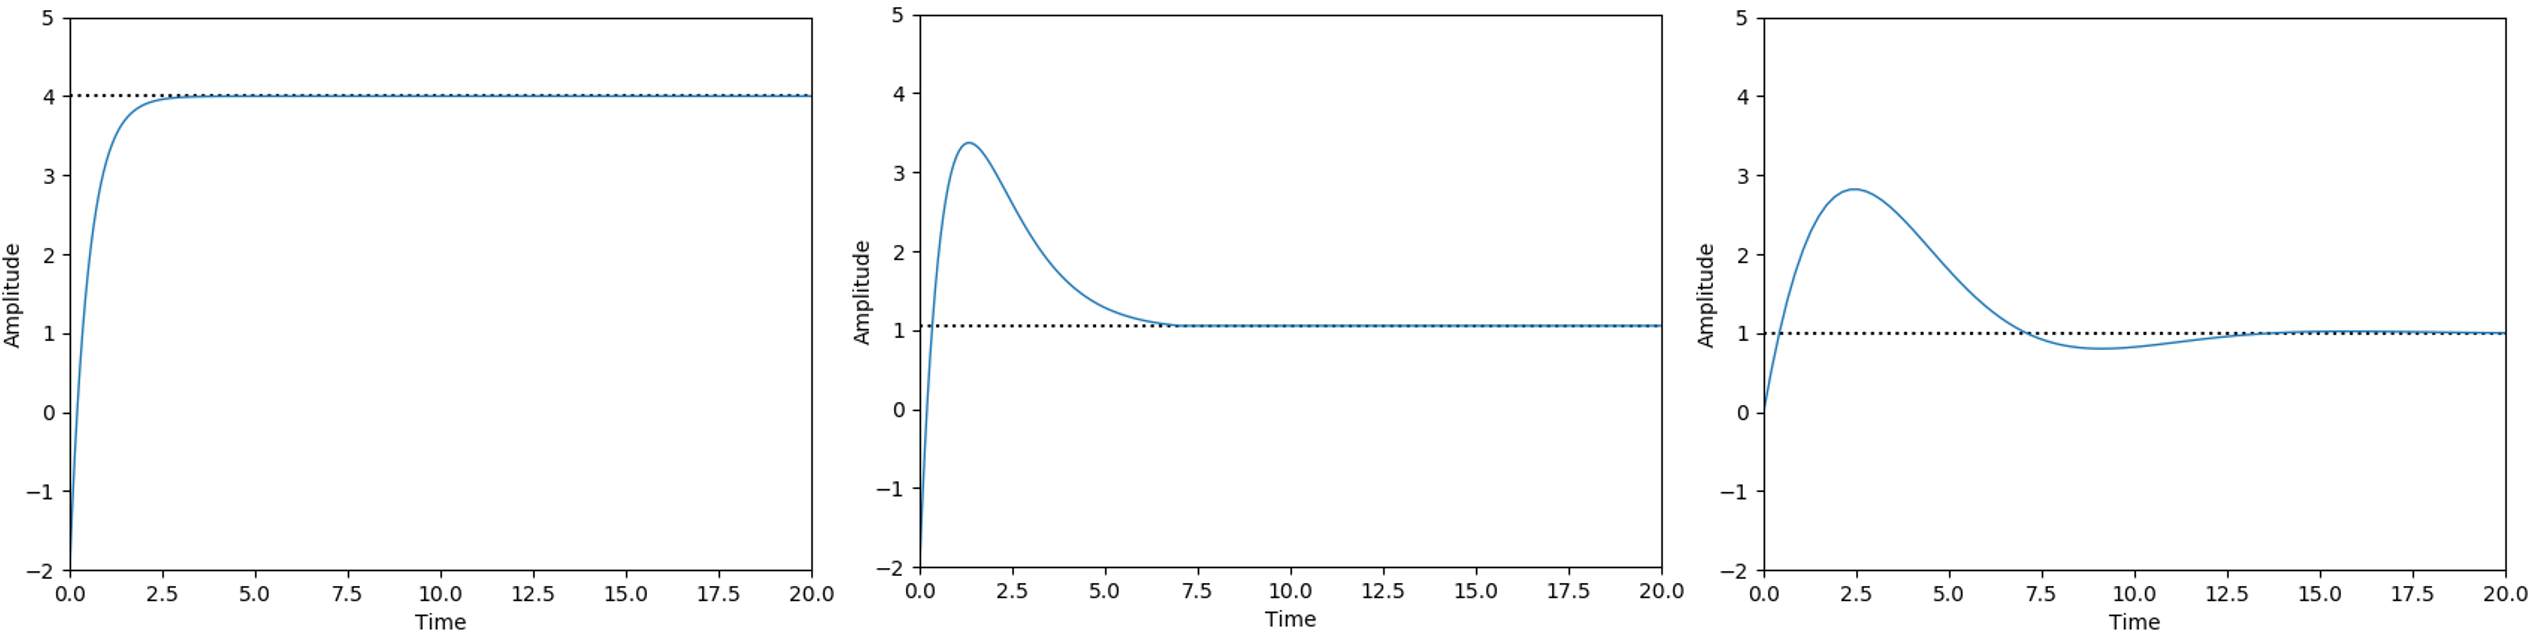
\includegraphics[scale=0.280]{img/longitudinal_control/Full-Size-Image.png}
\end{center}
\label{Full-Size-Image}
\end{figure}

	\begin{enumerate}
		\item 1st response by PI; 2nd response by PD; 3rd response by PID
		\item 1st response by PD; 2nd response by PI; 3rd response by PID
		\item 1st response by PI; 2nd response by PID; 3rd response by PD
		\item 1st response by PD; 2nd response by PID; 3rd response by PI
		\item None of the above
	\end{enumerate}
\item What is the output of a typical output of a Longitudinal control module? (Select all that apply)
	\begin{enumerate}
		\item  Reference velocity
		\item Throttle angle
		\item Steering angle
		\item Brake position
	\end{enumerate}
\item Based on the engine map in the figure below, determine the throttle angle needed to produce 
		250 ft-lb of torque given that the current engine speed is 3500 RPM.
\begin{figure}[!htb]
\begin{center}
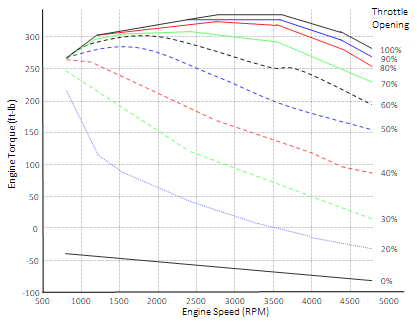
\includegraphics[scale=0.280]{img/longitudinal_control/image_q10.png}
\end{center}
\label{image_q10}
\end{figure}
		
\item The results of a simulation of the control response to a step change in desired speed of a dynamic vehicle model with a PID controller are shown in the figures below. 
There are two spikes on these figures: one spike is between 2 and 3 seconds, another spike is between 3 and 4 seconds. What is the reason of these spikes?
\begin{figure}[!htb]
\begin{center}
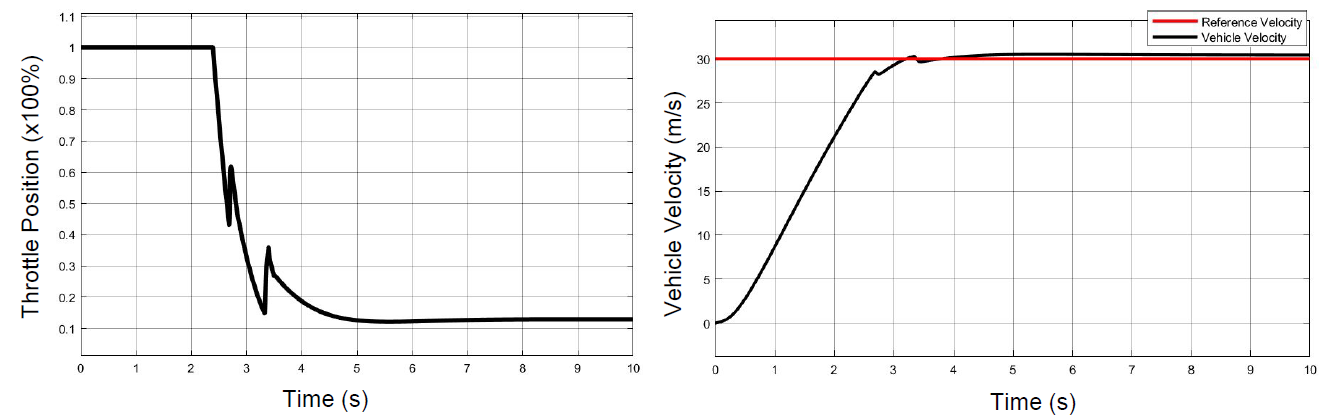
\includegraphics[scale=0.280]{img/longitudinal_control/image_q11.png}
\end{center}
\label{image_q11}
\end{figure}
	\begin{enumerate}
		\item  Engine-transmission torque loss
		\item Tire slip
		\item Nonlinear engine map
		\item High level controller simplification: changing the integral to a summation over fixed length time steps in the Integral term
		\item None of the above
	\end{enumerate}
\item What type of control system is shown in the figure below?
\begin{figure}[!htb]
\begin{center}
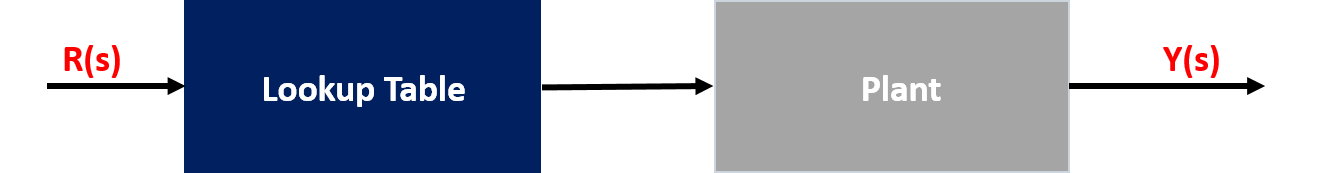
\includegraphics[scale=0.280]{img/longitudinal_control/Openloop.png}
\end{center}
\label{Openloop}
\end{figure}
	\begin{enumerate}
		\item  Feedback control
		\item Feedforward control
		\item Feedback-feedforward control
		\item None of the above
	\end{enumerate}
\item What types of inaccuracies are corrected by a feedback controller?
	\begin{enumerate}
		\item  Disturbances
		\item Nonlinear engine map
		\item Errors in the plant model
		\item High level controller simplification: changing the integral to a summation over fixed length time steps in the Integral term
	\end{enumerate}
\item What assumptions are essential for creation of a longitudinal feedforward input? (Select all that apply)
	\begin{enumerate}
		\item  The tire slip angle and ratio are negligible
		\item The vehicle is at steady state
		\item The plant system is linear
		\item Torque from the engine passes directly to the transmission without loss
	\end{enumerate}
\item What are the sources of the load torque considered for a longitudinal feedforward look-up table computation? (Select all that apply) 
	\begin{enumerate}
		\item   Rolling resistance
		\item Sliding resistance
		\item Gravitational resistance
		\item Cornering force
		\item Aerodynamic resistance
		\item Static friction
	\end{enumerate}
\item A vehicle is being operated on a highway with the reference velocity of $126km/h$ (35 m/s) 
in gear 4 and it overcomes the total load torque of 300 ft-lb. 
This vehicle specification includes effective wheel radius of 0.35 m and 4th gear ratio of 2. 
What throttle angle is required for maintaining the the current speed of the vehicle? Use the below engine map for your computation. 

\begin{figure}[!htb]
\begin{center}
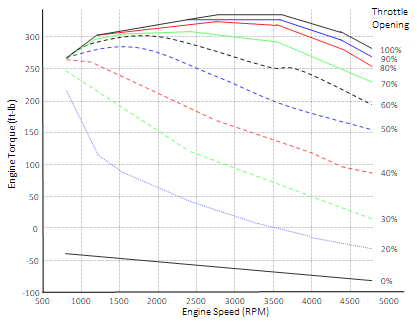
\includegraphics[scale=0.280]{img/longitudinal_control/image_q12.png}
\end{center}
\label{image_q12}
\end{figure}
\end{enumerate}


